\documentclass[aspectratio=169,11pt]{beamer}

% ========== PAQUETES ==========
\usepackage[utf8]{inputenc}
\usepackage[spanish,es-tabla]{babel}
\usepackage{graphicx}
\usepackage{xcolor}
\usepackage{tikz}
\usepackage{tcolorbox}
\usepackage{fontawesome5}
\usepackage{listings}
\usepackage{booktabs}
\usepackage{hyperref}
\usepackage{enumitem}

% ========== CONFIGURACIÓN DE COLORES UNSCH ==========
\definecolor{primaryblue}{RGB}{0,51,102}
\definecolor{secondaryblue}{RGB}{0,102,204}
\definecolor{accentgold}{RGB}{218,165,32}
\definecolor{lightgray}{RGB}{245,245,245}
\definecolor{darkgray}{RGB}{100,100,100}
\definecolor{successgreen}{RGB}{34,139,34}
\definecolor{warningred}{RGB}{178,34,34}

% ========== TEMA BEAMER ==========
\usetheme{Madrid}
\usecolortheme[named=primaryblue]{structure}

\setbeamercolor{frametitle}{bg=primaryblue,fg=white}
\setbeamercolor{title}{bg=primaryblue,fg=white}
\setbeamercolor{block title}{bg=secondaryblue,fg=white}
\setbeamercolor{block body}{bg=lightgray}

% ========== CAJAS PERSONALIZADAS ==========
\newtcolorbox{infobox}{
  colback=secondaryblue!5,
  colframe=secondaryblue,
  fonttitle=\bfseries,
  title=\faInfoCircle\ Información Importante,
  arc=3mm,
  boxrule=1.5pt
}

\newtcolorbox{warningbox}{
  colback=warningred!5,
  colframe=warningred,
  fonttitle=\bfseries,
  title=\faExclamationTriangle\ ¡Importante!,
  arc=3mm,
  boxrule=1.5pt
}

\newtcolorbox{successbox}{
  colback=successgreen!5,
  colframe=successgreen,
  fonttitle=\bfseries,
  title=\faCheckCircle\ Consejo Útil,
  arc=3mm,
  boxrule=1.5pt
}

\newtcolorbox{stepbox}[1]{
  colback=accentgold!10,
  colframe=accentgold,
  fonttitle=\bfseries,
  title=\faArrowRight\ #1,
  arc=2mm,
  boxrule=1.5pt
}

% ========== INFORMACIÓN DEL DOCUMENTO ==========
\title[Configuración Word APA 7]{Configuración de Microsoft Word\\con Normas APA 7ª Edición}
\subtitle{Plantillas para Monografía de Compilación e Investigación}
\author{Universidad Nacional de San Cristóbal de Huamanga}
\institute{Escuela de Ciencias de la Comunicación}
\date{2026}

% ========== INICIO DEL DOCUMENTO ==========
\begin{document}

% ========== PORTADA ==========
\begin{frame}
  \titlepage
  \begin{center}
    
\includegraphics[height=1cm]{images/cau-logo.png}
  \end{center}
\end{frame}

% ========== TABLA DE CONTENIDOS ==========
\begin{frame}{Contenido de la Clase}
  \tableofcontents
\end{frame}

% ========== SECCIÓN 1: INTRODUCCIÓN ==========
\section{Introducción al Taller}

\begin{frame}{Bienvenida al Taller}
  \begin{center}
    \Large \textbf{¡Bienvenidos!}\\[0.5cm]
    \normalsize Configuración de Word según Normas APA 7ª Edición
  \end{center}
  
  \vspace{0.5cm}
  
  \begin{block}{Objetivos del Taller}
    \begin{itemize}
      \item Configurar Microsoft Word paso a paso
      \item Crear plantilla para Monografía de Compilación
      \item Crear plantilla para Monografía de Investigación
      \item Automatizar índices, títulos y numeración
      \item Usar IA para generar estructura de contenidos
    \end{itemize}
  \end{block}
\end{frame}

\begin{frame}{¿Qué Aprenderás Hoy?}
  \begin{columns}[T]
    \column{0.5\textwidth}
    \textbf{\textcolor{primaryblue}{Configuración Técnica}}
    \begin{itemize}
      \item Márgenes y espaciado
      \item Fuentes y tamaños
      \item Encabezados y numeración
      \item Sangrías y alineación
      \item Estilos automáticos
    \end{itemize}
    
    \column{0.5\textwidth}
    \textbf{\textcolor{secondaryblue}{Herramientas Avanzadas}}
    \begin{itemize}
      \item Índices automáticos
      \item Referencias cruzadas
      \item Estilos personalizados
      \item Uso de IA para estructura
      \item Plantillas reutilizables
    \end{itemize}
  \end{columns}
\end{frame}

% ========== SECCIÓN 2: LINEAMIENTOS ==========
\section{Lineamientos de la Monografía}

\begin{frame}{Lineamientos Generales}
  \begin{center}
    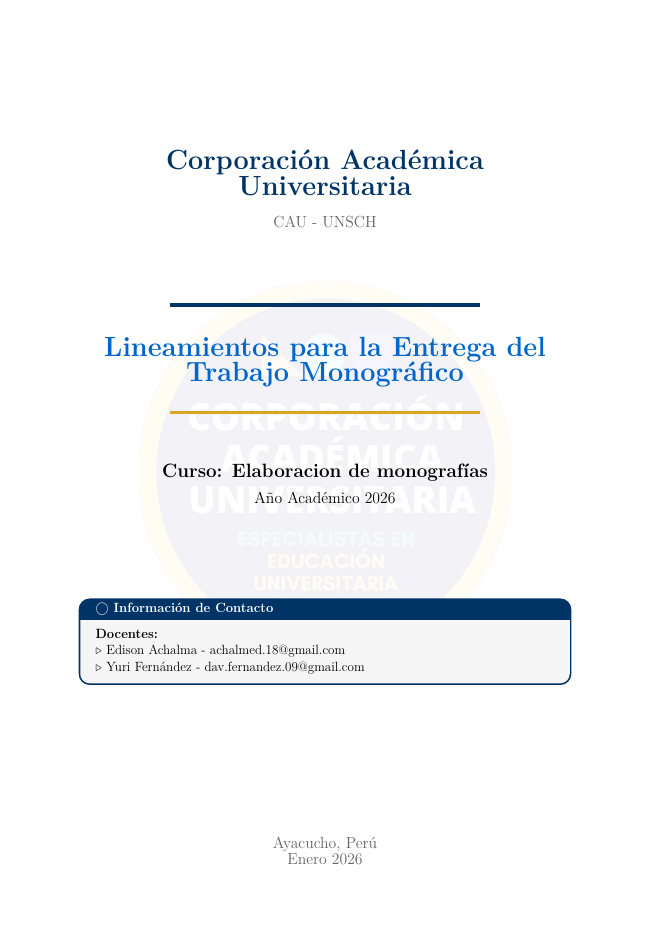
\includegraphics[width=0.85\textwidth]{images/lineamientos_portada.png}
  \end{center}
  
  \begin{warningbox}
    Descarga el PDF completo de lineamientos antes de comenzar
  \end{warningbox}
\end{frame}

\begin{frame}{Formato Según APA 7ª Edición}
  \begin{columns}[T]
    \column{0.5\textwidth}
    \textbf{\faFileAlt\ Papel y Márgenes}
    \begin{itemize}
      \item Tamaño: Carta (8.5" × 11")
      \item Márgenes: 2.54 cm todos los lados
      \item Una sola cara
    \end{itemize}
    
    \vspace{0.3cm}
    
    \textbf{\faFont\ Tipografía}
    \begin{itemize}
      \item Times New Roman 12 pt
      \item Calibri 11 pt (alternativa)
      \item Arial 11 pt (alternativa)
    \end{itemize}
    
    \column{0.5\textwidth}
    \textbf{\faAlignJustify\ Interlineado}
    \begin{itemize}
      \item Doble espacio (2.0)
      \item Sin espacio adicional entre párrafos
      \item Excepciones: tablas, figuras
    \end{itemize}
    
    \vspace{0.3cm}
    
    \textbf{\faListOl\ Numeración}
    \begin{itemize}
      \item Esquina superior derecha
      \item Todas las páginas
      \item Números arábigos
    \end{itemize}
  \end{columns}
\end{frame}

\begin{frame}{Diferencias: Compilación vs. Investigación}
  \begin{columns}[T]
    \column{0.48\textwidth}
    \begin{block}{Monografía de Compilación}
      \small
      \textbf{Características:}
      \begin{itemize}
        \item Análisis documental
        \item Revisión bibliográfica
        \item Síntesis de autores
        \item Sin trabajo de campo
        \item Cap. 3: Análisis comparativo
      \end{itemize}
    \end{block}
    
    \column{0.48\textwidth}
    \begin{block}{Monografía de Investigación}
      \small
      \textbf{Características:}
      \begin{itemize}
        \item Investigación empírica
        \item Recolección de datos
        \item Análisis de resultados
        \item Trabajo de campo
        \item Cap. 3: Metodología
        \item Cap. 4: Resultados
      \end{itemize}
    \end{block}
  \end{columns}
\end{frame}

% ========== SECCIÓN 3: CONFIGURACIÓN INICIAL ==========
\section{Configuración Inicial de Word}

\begin{frame}{Paso 1: Configurar Página}
  \begin{stepbox}{Configuración de Página}
    \textbf{Ruta:} Diseño → Márgenes → Márgenes personalizados
  \end{stepbox}
  
  \begin{center}
    \includegraphics[width=0.8\textwidth]{images/paso01_configurar_pagina.png}
  \end{center}
  
  \begin{enumerate}
    \item Abrir Microsoft Word
    \item Ir a pestaña \textbf{Diseño}
    \item Seleccionar \textbf{Márgenes personalizados}
  \end{enumerate}
\end{frame}

\begin{frame}{Paso 2: Establecer Márgenes}
  \begin{center}
    \includegraphics[width=0.65\textwidth]{images/paso02_margenes.png}
  \end{center}
  
  \begin{block}{Configuración de Márgenes APA}
    \begin{itemize}
      \item Superior: 2.54 cm (1 pulgada)
      \item Inferior: 2.54 cm (1 pulgada)
      \item Izquierdo: 2.54 cm (1 pulgada)
      \item Derecho: 2.54 cm (1 pulgada)
      \item Orientación: Vertical
    \end{itemize}
  \end{block}
\end{frame}

\begin{frame}{Paso 3: Configurar Fuente}
  \begin{center}
    \includegraphics[width=0.7\textwidth]{images/paso03_fuente.png}
  \end{center}
  
  \begin{columns}[T]
    \column{0.5\textwidth}
    \textbf{Opciones APA 7:}
    \begin{itemize}
      \item Times New Roman 12 pt
      \item Calibri 11 pt
      \item Arial 11 pt
    \end{itemize}
    
    \column{0.5\textwidth}
    \textbf{Recomendación:}\\
    \textcolor{successgreen}{Times New Roman 12 pt}\\
    (Más tradicional y académica)
  \end{columns}
  
  \vspace{0.3cm}
  
  \begin{successbox}
    Haz clic en ``Establecer como predeterminado'' para aplicar a todo el documento
  \end{successbox}
\end{frame}

\begin{frame}{Paso 4: Configurar Interlineado}
  \begin{center}
    \includegraphics[width=0.7\textwidth]{images/paso04_interlineado.png}
  \end{center}
  
  \begin{warningbox}
    \textbf{Configuración Crítica:}
    \begin{itemize}
      \item Interlineado: \textbf{Doble (2.0)}
      \item Espaciado anterior: \textbf{0 pt}
      \item Espaciado posterior: \textbf{0 pt}
      \item Alineación: \textbf{Justificada}
    \end{itemize}
  \end{warningbox}
\end{frame}

\begin{frame}{Paso 5: Configurar Sangría}
  \begin{center}
    \includegraphics[width=0.75\textwidth]{images/paso05_sangria.png}
  \end{center}
  
  \begin{block}{Sangría de Primera Línea}
    \begin{itemize}
      \item Ir a \textbf{Inicio → Párrafo}
      \item En \textbf{Sangría especial}: seleccionar ``Primera línea''
      \item Valor: \textbf{1.27 cm (0.5 pulgadas)}
      \item Aplicar a todo el documento
    \end{itemize}
  \end{block}
\end{frame}

% ========== SECCIÓN 4: NUMERACIÓN Y ENCABEZADOS ==========
\section{Numeración y Encabezados}

\begin{frame}{Paso 6: Insertar Número de Página}
  \begin{center}
    \includegraphics[width=0.8\textwidth]{images/paso06_numero_pagina.png}
  \end{center}
  
  \begin{stepbox}{Numeración de Páginas}
    \begin{enumerate}
      \item \textbf{Insertar → Número de página}
      \item Seleccionar: \textbf{Principio de página → Número sin formato 3}
      \item Ubicación: Esquina superior derecha
    \end{enumerate}
  \end{stepbox}
\end{frame}

\begin{frame}{Paso 7: Running Head (Opcional)}
  \begin{center}
    \includegraphics[width=0.75\textwidth]{images/paso07_running_head.png}
  \end{center}
  
  \begin{warningbox}
    \textbf{Nota APA 7:} El running head NO es requerido para trabajos estudiantiles.\\
    Solo para trabajos profesionales (publicaciones).
  \end{warningbox}
  
  \begin{block}{Si tu institución lo requiere:}
    \begin{itemize}
      \item Máximo 50 caracteres
      \item Todo en MAYÚSCULAS
      \item Alineado a la izquierda
    \end{itemize}
  \end{block}
\end{frame}

% ========== SECCIÓN 5: ESTILOS AUTOMÁTICOS ==========
\section{Estilos y Títulos Automáticos}

\begin{frame}{¿Por Qué Usar Estilos?}
  \begin{center}
    \Large \textbf{Beneficios de los Estilos Automáticos}
  \end{center}
  
  \vspace{0.5cm}
  
  \begin{columns}[T]
    \column{0.5\textwidth}
    \textbf{\textcolor{successgreen}{CON Estilos}}
    \begin{itemize}
      \item[\faCheckCircle] Formato consistente
      \item[\faCheckCircle] Índice automático
      \item[\faCheckCircle] Navegación fácil
      \item[\faCheckCircle] Actualización rápida
      \item[\faCheckCircle] Ahorro de tiempo
    \end{itemize}
    
    \column{0.5\textwidth}
    \textbf{\textcolor{warningred}{SIN Estilos}}
    \begin{itemize}
      \item[\faTimesCircle] Formato manual
      \item[\faTimesCircle] Índice manual
      \item[\faTimesCircle] Difícil navegación
      \item[\faTimesCircle] Errores frecuentes
      \item[\faTimesCircle] Pérdida de tiempo
    \end{itemize}
  \end{columns}
\end{frame}

\begin{frame}{Niveles de Títulos en APA 7}
  \begin{center}
    \includegraphics[width=0.9\textwidth]{images/niveles_titulos_apa.png}
  \end{center}
  
  \small
  \begin{tabular}{|l|p{8cm}|}
    \hline
    \textbf{Nivel} & \textbf{Formato} \\
    \hline
    1 & Centrado, Negrita, Título Capitalizado \\
    \hline
    2 & Alineado Izq., Negrita, Título Capitalizado \\
    \hline
    3 & Alineado Izq., Negrita Cursiva, Título Capitalizado \\
    \hline
    4 & Sangría, Negrita, Título Cap., punto final. Texto sigue... \\
    \hline
    5 & Sangría, Negrita Cursiva, Título Cap., punto. Texto... \\
    \hline
  \end{tabular}
\end{frame}

\begin{frame}{Paso 8: Configurar Estilo Título 1}
  \begin{center}
    \includegraphics[width=0.75\textwidth]{images/paso08_titulo1.png}
  \end{center}
  
  \begin{block}{Configuración Título 1}
    \begin{itemize}
      \item \textbf{Ruta:} Inicio → Estilos → Título 1 (clic derecho) → Modificar
      \item Fuente: Times New Roman, 12 pt, Negrita
      \item Alineación: Centrado
      \item Espaciado: Anterior 0 pt, Posterior 0 pt
      \item Interlineado: Doble
    \end{itemize}
  \end{block}
\end{frame}

\begin{frame}{Paso 9: Configurar Estilo Título 2}
  \begin{center}
    \includegraphics[width=0.75\textwidth]{images/paso09_titulo2.png}
  \end{center}
  
  \begin{block}{Configuración Título 2}
    \begin{itemize}
      \item Fuente: Times New Roman, 12 pt, Negrita
      \item Alineación: Izquierda
      \item Espaciado: Anterior 0 pt, Posterior 0 pt
      \item Interlineado: Doble
    \end{itemize}
  \end{block}
\end{frame}

\begin{frame}{Paso 10: Configurar Estilo Título 3}
  \begin{center}
    \includegraphics[width=0.75\textwidth]{images/paso10_titulo3.png}
  \end{center}
  
  \begin{block}{Configuración Título 3}
    \begin{itemize}
      \item Fuente: Times New Roman, 12 pt, Negrita, \textit{Cursiva}
      \item Alineación: Izquierda
      \item Espaciado: Anterior 0 pt, Posterior 0 pt
      \item Interlineado: Doble
    \end{itemize}
  \end{block}
\end{frame}

% ========== SECCIÓN 6: USO DE IA ==========
\section{Generación de Estructura con IA}

\begin{frame}{Uso de IA para Generar Títulos y Estructura}
  \begin{center}
    \includegraphics[width=0.8\textwidth]{images/ia_herramientas.png}
  \end{center}
  
  \begin{block}{\faRobot\ Herramientas de IA Recomendadas}
    \begin{itemize}
      \item ChatGPT (OpenAI) - GPT-4
      \item Claude AI (Anthropic)
      \item Perplexity AI
      \item Gemini (Google)
    \end{itemize}
  \end{block}
\end{frame}

\begin{frame}[fragile]{Prompt para Monografía de Compilación}
  \begin{stepbox}{Ejemplo de Prompt para IA}
  \end{stepbox}
  
  \begin{tcolorbox}[colback=lightgray,colframe=darkgray,fontsize=\tiny]
\begin{verbatim}
Actúa como experto en [tu carrera profesional]. 
Necesito que me generes una estructura detallada para una 
monografía de COMPILACIÓN sobre:

TEMA: [INSERTA TU TEMA AQUÍ]
ÁREA: Ciencias de la Comunicación
TIPO: Monografía de compilación (revisión bibliográfica)

Genera una estructura con:
- Capítulo 1: Introducción (con 3-4 subtítulos)
- Capítulo 2: Marco Teórico (con 5-6 subtítulos temáticos)
- Capítulo 3: Análisis Comparativo (con 4-5 subtítulos)
- Conclusiones
- Recomendaciones

Los títulos deben ser específicos, relevantes y académicos.
\end{verbatim}
  \end{tcolorbox}
\end{frame}

\begin{frame}[fragile]{Prompt para Monografía de Investigación}
  \begin{stepbox}{Ejemplo de Prompt para IA}
  \end{stepbox}
  
  \begin{tcolorbox}[colback=lightgray,colframe=darkgray,fontsize=\tiny]
\begin{verbatim}
Actúa como experto en [tu carrera profesional]. 
Necesito que me generes una estructura detallada para una 
monografía de INVESTIGACIÓN sobre:

TEMA: [INSERTA TU TEMA AQUÍ]
ÁREA: Ciencias de la Comunicación
TIPO: Monografía de investigación (trabajo de campo)

Genera una estructura con:
- Capítulo 1: Introducción (con 3-4 subtítulos)
- Capítulo 2: Marco Teórico (con 5-6 subtítulos)
- Capítulo 3: Metodología (tipo, técnicas, instrumentos, procedimiento)
- Capítulo 4: Resultados y Análisis (con 4-5 subtítulos)
- Conclusiones
- Recomendaciones

Los títulos deben ser específicos, relevantes y académicos.
\end{verbatim}
  \end{tcolorbox}
\end{frame}

\begin{frame}{Ejemplo de Respuesta de IA}
  \begin{center}
    \includegraphics[width=0.85\textwidth]{images/ejemplo_ia_respuesta.png}
  \end{center}
  
  \begin{successbox}
    Copia la estructura generada y pégala en tu documento Word, luego aplica los estilos de título correspondientes.
  \end{successbox}
\end{frame}

\begin{frame}{Paso 11: Aplicar Estilos a Estructura Generada}
  \begin{center}
    \includegraphics[width=0.8\textwidth]{images/paso11_aplicar_estilos.png}
  \end{center}
  
  \begin{stepbox}{Formatear Títulos con Estilos}
    Para cada título generado por IA:
    \begin{enumerate}
      \item Selecciona el texto del título
      \item Aplica el estilo correspondiente:
      \begin{itemize}
        \item Capítulos principales → Título 1
        \item Secciones → Título 2
        \item Subsecciones → Título 3
      \end{itemize}
    \end{enumerate}
  \end{stepbox}
\end{frame}

% ========== SECCIÓN 7: ÍNDICE AUTOMÁTICO ==========
\section{Tabla de Contenido Automática}

\begin{frame}{Paso 12: Crear Tabla de Contenido}
  \begin{center}
    \includegraphics[width=0.8\textwidth]{images/paso12_tabla_contenido.png}
  \end{center}
  
  \begin{stepbox}{Insertar Índice Automático}
    \begin{enumerate}
      \item Posicionar cursor donde irá el índice
      \item \textbf{Referencias → Tabla de contenido}
      \item Seleccionar: \textbf{Tabla automática 1}
    \end{enumerate}
  \end{stepbox}
  
  \begin{successbox}
    Al usar estilos de título, el índice se genera automáticamente.
  \end{successbox}
\end{frame}

\begin{frame}{Personalizar Tabla de Contenido}
  \begin{center}
    \includegraphics[width=0.7\textwidth]{images/paso12_personalizar_indice.png}
  \end{center}
  
  \begin{block}{Opciones Recomendadas}
    \begin{itemize}
      \item Mostrar números de página: ✓
      \item Alinear números a la derecha: ✓
      \item Carácter de relleno: Puntos (.......)
      \item Mostrar niveles: 3
      \item Formato: De la plantilla
    \end{itemize}
  \end{block}
\end{frame}

\begin{frame}{Actualizar Tabla de Contenido}
  \begin{center}
    \includegraphics[width=0.75\textwidth]{images/paso13_actualizar_indice.png}
  \end{center}
  
  \begin{warningbox}
    \textbf{Importante:} Cada vez que agregues o modifiques títulos:
    \begin{enumerate}
      \item Clic derecho en la tabla de contenido
      \item Seleccionar \textbf{Actualizar campos}
      \item Elegir \textbf{Actualizar toda la tabla}
    \end{enumerate}
  \end{warningbox}
\end{frame}

% ========== SECCIÓN 8: PORTADAS ==========
\section{Configuración de Portadas}

\begin{frame}{Elementos de la Portada}
  \begin{center}
    \includegraphics[width=0.65\textwidth]{images/portada_ejemplo.png}
  \end{center}
  
  \begin{block}{Elementos Requeridos (APA 7 - Estudiantes)}
    \begin{enumerate}
      \item Título del trabajo (negrita, centrado)
      \item Nombre del autor
      \item Afiliación institucional
      \item Número y nombre del curso
      \item Nombre del instructor
      \item Fecha de entrega
    \end{enumerate}
  \end{block}
\end{frame}

\begin{frame}{Paso 14: Crear Portada}
  \begin{center}
    \includegraphics[width=0.8\textwidth]{images/paso14_crear_portada.png}
  \end{center}
  
  \begin{stepbox}{Configuración de Portada}
    \begin{enumerate}
      \item Insertar página en blanco al inicio
      \item Centrar verticalmente el contenido
      \item Aplicar formato según APA 7
      \item Sin número de página en portada
    \end{enumerate}
  \end{stepbox}
\end{frame}

% ========== SECCIÓN 9: REFERENCIAS ==========
\section{Referencias Bibliográficas}

\begin{frame}{Gestión de Referencias en Word}
  \begin{center}
    \includegraphics[width=0.8\textwidth]{images/paso15_referencias.png}
  \end{center}
  
  \begin{block}{Herramientas en Word}
    \begin{itemize}
      \item \textbf{Referencias → Estilo → APA 7th edition}
      \item Insertar cita
      \item Administrar fuentes
      \item Bibliografía automática
    \end{itemize}
  \end{block}
\end{frame}

\begin{frame}{Paso 15: Configurar Estilo APA 7}
  \begin{center}
    \includegraphics[width=0.8\textwidth]{images/paso15_estilo_apa7.png}
  \end{center}
  
  \begin{warningbox}
    \textbf{Crítico:} Asegúrate de seleccionar \textbf{APA 7th edition}\\
    NO APA 6th edition
  \end{warningbox}
\end{frame}

\begin{frame}{Paso 16: Insertar Citas en el Texto}
  \begin{center}
    \includegraphics[width=0.8\textwidth]{images/paso16_insertar_citas.png}
  \end{center}
  
  \begin{block}{Tipos de Citas APA 7}
    \begin{itemize}
      \item Cita narrativa: Autor (año)
      \item Cita parentética: (Autor, año)
      \item Cita con página: (Autor, año, p. XX)
      \item Cita directa: ``texto'' (Autor, año, p. XX)
    \end{itemize}
  \end{block}
\end{frame}

\begin{frame}{Paso 17: Generar Lista de Referencias}
  \begin{center}
    \includegraphics[width=0.8\textwidth]{images/paso17_bibliografia.png}
  \end{center}
  
  \begin{stepbox}{Crear Bibliografía Automática}
    \begin{enumerate}
      \item Posicionar cursor al final del documento
      \item \textbf{Referencias → Bibliografía}
      \item Seleccionar: \textbf{Referencias}
      \item Se genera automáticamente con formato APA 7
    \end{enumerate}
  \end{stepbox}
\end{frame}

% ========== SECCIÓN 10: PLANTILLA COMPILACIÓN ==========
\section{Plantilla: Monografía de Compilación}

\begin{frame}{Estructura - Monografía de Compilación}
  \begin{center}
    \includegraphics[width=0.8\textwidth]{images/estructura_compilacion.png}
  \end{center}
  
  \begin{block}{Capítulos Principales}
    \begin{enumerate}
      \item Capítulo 1: Anotaciones Preliminares
      \item Capítulo 2: Marco Teórico
      \item Capítulo 3: Análisis Comparativo de Autores
      \item Conclusiones
      \item Recomendaciones
    \end{enumerate}
  \end{block}
\end{frame}

\begin{frame}{Configuración Específica - Compilación}
  \begin{center}
    \includegraphics[width=0.75\textwidth]{images/plantilla_compilacion.png}
  \end{center}
  
  \begin{block}{Elementos Específicos}
    \begin{itemize}
      \item Sección de antecedentes
      \item Justificación del tema
      \item Descripción y delimitación
      \item Objetivos
      \item Marco teórico extenso
      \item Análisis comparativo de autores
    \end{itemize}
  \end{block}
\end{frame}

\begin{frame}[fragile]{Ejemplo: Capítulo 3 - Compilación}
  \begin{block}{Análisis Comparativo}
    \small
\begin{verbatim}
3. ANÁLISIS COMPARATIVO

3.1 Principales Enfoques Teóricos
    3.1.1 Perspectiva de [Autor 1]
    3.1.2 Perspectiva de [Autor 2]
    3.1.3 Perspectiva de [Autor 3]

3.2 Puntos de Convergencia

3.3 Puntos de Divergencia

3.4 Síntesis Integradora
\end{verbatim}
  \end{block}
\end{frame}

% ========== SECCIÓN 11: PLANTILLA INVESTIGACIÓN ==========
\section{Plantilla: Monografía de Investigación}

\begin{frame}{Estructura - Monografía de Investigación}
  \begin{center}
    \includegraphics[width=0.8\textwidth]{images/estructura_investigacion.png}
  \end{center}
  
  \begin{block}{Capítulos Principales}
    \begin{enumerate}
      \item Capítulo 1: Anotaciones Preliminares
      \item Capítulo 2: Marco Teórico
      \item Capítulo 3: Metodología
      \item Capítulo 4: Resultados y Análisis
      \item Conclusiones
      \item Recomendaciones
    \end{enumerate}
  \end{block}
\end{frame}

\begin{frame}{Configuración Específica - Investigación}
  \begin{center}
    \includegraphics[width=0.75\textwidth]{images/plantilla_investigacion.png}
  \end{center}
  
  \begin{block}{Elementos Adicionales}
    \begin{itemize}
      \item Planteamiento del problema
      \item Hipótesis (si aplica)
      \item Diseño metodológico
      \item Instrumentos de recolección
      \item Presentación de resultados
      \item Discusión de hallazgos
    \end{itemize}
  \end{block}
\end{frame}

\begin{frame}[fragile]{Ejemplo: Capítulo 3 - Investigación}
  \begin{block}{Metodología}
    \small
\begin{verbatim}
3. METODOLOGÍA

3.1 Tipo de Investigación

3.2 Diseño de Investigación

3.3 Población y Muestra

3.4 Técnicas e Instrumentos
    3.4.1 Técnicas de recolección
    3.4.2 Instrumentos utilizados

3.5 Procedimiento
\end{verbatim}
  \end{block}
\end{frame}

\begin{frame}[fragile]{Ejemplo: Capítulo 4 - Resultados}
  \begin{block}{Resultados y Análisis}
    \small
\begin{verbatim}
4. RESULTADOS Y ANÁLISIS

4.1 Presentación de Resultados
    4.1.1 Datos descriptivos
    4.1.2 Datos inferenciales

4.2 Análisis de Resultados
    4.2.1 Análisis por objetivo 1
    4.2.2 Análisis por objetivo 2

4.3 Discusión de Hallazgos

4.4 Contrastación con Marco Teórico
\end{verbatim}
  \end{block}
\end{frame}

% ========== SECCIÓN 12: TABLAS Y FIGURAS ==========
\section{Tablas y Figuras APA 7}

\begin{frame}{Formato de Tablas APA 7}
  \begin{center}
    \includegraphics[width=0.8\textwidth]{images/tabla_apa_ejemplo.png}
  \end{center}
  
  \begin{block}{Elementos de una Tabla}
    \begin{enumerate}
      \item Número de tabla (Tabla 1, Tabla 2...)
      \item Título descriptivo en cursiva
      \item Cuerpo de la tabla
      \item Notas (si son necesarias)
    \end{enumerate}
  \end{block}
\end{frame}

\begin{frame}{Paso 18: Insertar y Formatear Tablas}
  \begin{center}
    \includegraphics[width=0.8\textwidth]{images/paso18_insertar_tabla.png}
  \end{center}
  
  \begin{warningbox}
    \textbf{Reglas APA 7 para Tablas:}
    \begin{itemize}
      \item Sin bordes verticales
      \item Líneas horizontales solo arriba y abajo
      \item Números y títulos arriba de la tabla
      \item Notas abajo de la tabla
      \item Fuente del mismo tamaño que el texto
    \end{itemize}
  \end{warningbox}
\end{frame}

\begin{frame}{Formato de Figuras APA 7}
  \begin{center}
    \includegraphics[width=0.65\textwidth]{images/figura_apa_ejemplo.png}
  \end{center}
  
  \begin{block}{Elementos de una Figura}
    \begin{enumerate}
      \item Número de figura (Figura 1, Figura 2...)
      \item Título descriptivo en cursiva
      \item La imagen/gráfico
      \item Notas (si son necesarias)
    \end{enumerate}
  \end{block}
\end{frame}

\begin{frame}{Paso 19: Insertar y Formatear Figuras}
  \begin{center}
    \includegraphics[width=0.8\textwidth]{images/paso19_insertar_figura.png}
  \end{center}
  
  \begin{block}{Reglas APA 7 para Figuras}
    \begin{itemize}
      \item Números y títulos debajo de la figura
      \item Resolución mínima: 300 dpi
      \item Tamaño legible
      \item Notas debajo del título
      \item Referencia en el texto antes de aparecer
    \end{itemize}
  \end{block}
\end{frame}

% ========== SECCIÓN 13: CONSEJOS FINALES ==========
\section{Consejos y Mejores Prácticas}

\begin{frame}{Errores Comunes a Evitar}
  \begin{columns}[T]
    \column{0.5\textwidth}
    \textbf{\textcolor{warningred}{NO Hacer}}
    \begin{itemize}
      \item[\faTimesCircle] Usar Enter para espaciar
      \item[\faTimesCircle] Espacios manuales
      \item[\faTimesCircle] Cambiar formato a mano
      \item[\faTimesCircle] Tablas sin formato APA
      \item[\faTimesCircle] Índice manual
      \item[\faTimesCircle] Mezclar fuentes
      \item[\faTimesCircle] Ignorar estilos
    \end{itemize}
    
    \column{0.5\textwidth}
    \textbf{\textcolor{successgreen}{SÍ Hacer}}
    \begin{itemize}
      \item[\faCheckCircle] Usar estilos de párrafo
      \item[\faCheckCircle] Configurar bien desde inicio
      \item[\faCheckCircle] Usar índice automático
      \item[\faCheckCircle] Actualizar referencias
      \item[\faCheckCircle] Revisar formato APA
      \item[\faCheckCircle] Guardar como plantilla
      \item[\faCheckCircle] Hacer copias de respaldo
    \end{itemize}
  \end{columns}
\end{frame}

\begin{frame}{Checklist de Verificación Final}
  \begin{block}{\faCheckSquare\ Lista de Verificación}
    \begin{itemize}
      \item[$\square$] Márgenes correctos (2.54 cm todos los lados)
      \item[$\square$] Fuente Times New Roman 12 pt
      \item[$\square$] Interlineado doble en todo el documento
      \item[$\square$] Sangría primera línea 1.27 cm
      \item[$\square$] Números de página en esquina superior derecha
      \item[$\square$] Estilos de títulos aplicados correctamente
      \item[$\square$] Índice actualizado
      \item[$\square$] Referencias en formato APA 7
      \item[$\square$] Tablas y figuras numeradas y formateadas
      \item[$\square$] Portada con todos los elementos
    \end{itemize}
  \end{block}
\end{frame}

\begin{frame}{Paso 20: Guardar como Plantilla}
  \begin{center}
    \includegraphics[width=0.8\textwidth]{images/paso20_guardar_plantilla.png}
  \end{center}
  
  \begin{stepbox}{Guardar Documento como Plantilla}
    \begin{enumerate}
      \item \textbf{Archivo → Guardar como}
      \item Tipo de archivo: \textbf{Plantilla de Word (*.dotx)}
      \item Nombre sugerido:
      \begin{itemize}
        \item ``Plantilla\_Monografia\_Compilacion\_APA7.dotx''
        \item ``Plantilla\_Monografia\_Investigacion\_APA7.dotx''
      \end{itemize}
      \item Guardar en carpeta accesible
    \end{enumerate}
  \end{stepbox}
\end{frame}

\begin{frame}{Recursos Adicionales}
  \begin{block}{\faBook\ Bibliografía Recomendada}
    \begin{itemize}
      \item American Psychological Association. (2020). \textit{Publication Manual} (7th ed.)
      \item Manual de estilo UNSCH
      \item Lineamientos de monografía
    \end{itemize}
  \end{block}
  
  \begin{block}{\faGlobe\ Recursos en Línea}
    \begin{itemize}
      \item \url{https://apastyle.apa.org}
      \item \url{https://aracellymerida.wordpress.com}
      \item Tutorial en video: \url{https://youtu.be/e0xcJZJxAVQ}
    \end{itemize}
  \end{block}
\end{frame}

% ========== SECCIÓN 14: PRÁCTICA ==========
\section{Actividad Práctica}

\begin{frame}{Actividad Práctica en Clase}
  \begin{center}
    \Large \textbf{¡Ahora es tu turno!}
  \end{center}
  
  \vspace{0.5cm}
  
  \begin{block}{Tarea para Realizar Ahora}
    \begin{enumerate}
      \item Abre Microsoft Word
      \item Configura márgenes, fuente e interlineado
      \item Crea los 3 estilos de título
      \item Usa IA para generar estructura de tu tema
      \item Inserta la estructura en Word
      \item Aplica los estilos
      \item Genera tabla de contenido
      \item Crea la portada
      \item Guarda como plantilla
    \end{enumerate}
  \end{block}
  
  \begin{warningbox}
    Tiempo estimado: 45-60 minutos
  \end{warningbox}
\end{frame}

\begin{frame}{Temas Disponibles por Carrera}
  \begin{center}
    \includegraphics[width=0.85\textwidth]{images/temas_por_carrera.png}
  \end{center}
  
  \begin{infobox}
    Cada estudiante recibirá una lista de temas sugeridos según su carrera profesional
  \end{infobox}
\end{frame}

\begin{frame}{Entrega de Plantillas}
  \begin{block}{¿Qué entregar?}
    Al finalizar la clase, cada estudiante debe enviar:
    
    \begin{enumerate}
      \item Plantilla de Monografía (según su tipo)
      \item Con estructura generada por IA
      \item Estilos configurados
      \item Índice automático funcionando
      \item Portada completa
    \end{enumerate}
  \end{block}
  
  \begin{warningbox}
    \textbf{Formato de entrega:}
    \begin{itemize}
      \item Archivo: Apellido\_Plantilla\_Monografia.dotx
      \item Enviar a: [correo del profesor]
      \item Asunto: Plantilla Monografía - [Tu nombre]
    \end{itemize}
  \end{warningbox}
\end{frame}

% ========== PREGUNTAS ==========
\begin{frame}{Preguntas y Respuestas}
  \begin{center}
    \Huge \faQuestionCircle
    
    \vspace{1cm}
    
    \Large ¿Preguntas?
    
    \vspace{1cm}
    
    \normalsize
    Ahora es el momento de aclarar\\
    cualquier duda que tengas
  \end{center}
\end{frame}

% ========== CONTACTO ==========
\begin{frame}{Información de Contacto}
  \begin{center}
    \includegraphics[width=0.15\textwidth]{images/qr_contacto.png}
  \end{center}
  
  \begin{block}{Contacto}
    \begin{itemize}
      \item \faEnvelope\ [correo@universidad.edu]
      \item \faGlobe\ \url{https://aracellymerida.wordpress.com}
      \item \faYoutube\ Canal YouTube
      \item \faGithub\ GitHub: [usuario]
    \end{itemize}
  \end{block}
  
  \begin{center}
    \textbf{Horario de consultas:}\\
    Lunes a Viernes, 2:00 PM - 4:00 PM
  \end{center}
\end{frame}

% ========== CIERRE ==========
\begin{frame}[plain]
  \begin{center}
    {\Huge \textcolor{primaryblue}{\textbf{¡Gracias!}}}
    
    \vspace{1cm}
    
    {\Large Mucho éxito con sus monografías}
    
    \vspace{1cm}
    
    \normalsize
    \textit{``La excelencia en la escritura es crítica para el éxito\\
    en muchas actividades académicas y profesionales''}
    
    \vspace{0.5cm}
    
    --- American Psychological Association
    
    \vspace{1cm}
    
    \includegraphics[width=0.25\textwidth]{images/logo_unsch.png}
  \end{center}
\end{frame}

\end{document}
